\documentclass[11pt]{article}
\usepackage[margin=1in]{geometry}
\usepackage{amsmath,amssymb,amsthm,mathtools}
\usepackage{graphicx}
\usepackage{microtype}
\usepackage[colorlinks=true,linkcolor=blue,citecolor=blue,urlcolor=blue]{hyperref}

\newtheorem{theorem}{Theorem}
\newtheorem{lemma}{Lemma}
\newtheorem{corollary}{Corollary}
\newcommand{\D}{\mathbb D}
\newcommand{\hinf}{H^\infty}

\title{Every nonzero bounded companion operator on $H^\infty$\\
fixes a copy of $\ell^\infty$}
\author{Run \texttt{fa\_banach\_001}, lane 17
  (\texttt{agent\_lane\_17})}
\date{13 August 2026}

\begin{document}
\maketitle

\begin{abstract}
For $g$ analytic on the disk, let
$S_gf(z)=\int_0^z f'(w)g(w)\,dw$.  Lin, Liu, and Wu ask whether every bounded
noncompact $S_g:H^\infty\to H^\infty$ fixes an isomorphic copy of
$\ell^\infty$.  We prove the stronger statement that every nonzero bounded
$S_g$ does so.  The copy is produced by derivative interpolation on a
geometrically separated sequence along which $g$ is bounded below.  This
also makes compactness, weak compactness, strict singularity, and the zero
symbol equivalent for bounded companion operators on $H^\infty$.
\end{abstract}

\begin{center}
\fbox{\parbox{0.91\textwidth}{
\textbf{Status: full affirmative answer, likely valid, pending human review.}
No later explicit resolution was found in the bounded search described
below.
}}
\end{center}

\section{Exact source question}

For $g\in H(\D)$, define
\[
 (S_gf)(z)=\int_0^z f'(w)g(w)\,dw,
 \qquad f\in H(\D).
\]
Section 5, printed/PDF page 7 of Lin--Liu--Wu, arXiv:1903.10261v3
\cite{LLW}, asks:
\begin{quote}
Suppose that $S_g:H^\infty\to H^\infty$ is bounded but not compact.  Does
$S_g$ fix an isomorphic copy of $\ell^\infty$?  In particular, is $S_g$ not
strictly singular?
\end{quote}
The exact source passage is reproduced here:
\begin{center}

\includegraphics[width=0.97\textwidth]{figures/open_question_crop.png}
\end{center}

Anderson--Jovovic--Smith independently prove that the only compact companion
operator on $H^\infty$ is the zero operator \cite[Proposition 3.3]{AJS}:
\begin{center}
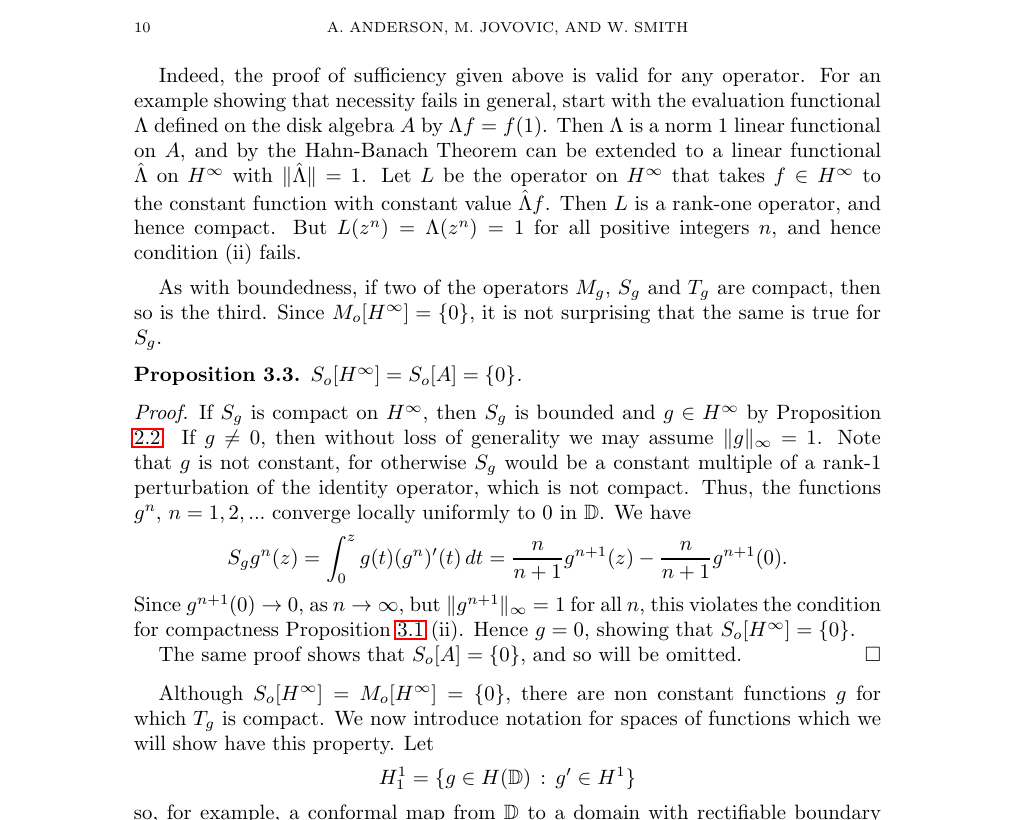
\includegraphics[width=0.91\textwidth]{figures/supporting_compactness_crop.png}
\end{center}
The proof below recovers that fact while resolving the stronger fixing
question.

\section{Proof intuition}

The derivative identity
\begin{equation}\label{eq:derivative}
 (S_gf)'=gf'
\end{equation}
suggests encoding an arbitrary bounded scalar sequence in normalized
derivatives of bounded analytic functions.  Choose points $z_n$ tending to
the boundary so quickly that they form an $H^\infty$ interpolating sequence,
while choosing their arguments so that $|g(z_n)|$ stays uniformly positive.
An interpolating Blaschke product forces the constructed functions to vanish
at every $z_n$, and ordinary value interpolation then prescribes their first
derivatives.  Equation \eqref{eq:derivative} multiplies the encoded coordinate
by $g(z_n)$.  The Schwarz--Pick derivative bound converts those coordinates
back into a lower bound for the $H^\infty$ norm.

\section{Three elementary ingredients}

We repeatedly use the following consequence of Schwarz--Pick:
\begin{equation}\label{eq:SP}
 (1-|z|^2)|h'(z)|\le \|h\|_\infty,
 \qquad h\in H^\infty, z\in\D.
\end{equation}

\begin{lemma}[The symbol is bounded]\label{lem:symbol}
If $S_g:H^\infty\to H^\infty$ is bounded, then
$g\in H^\infty$ and $\|g\|_\infty\le\|S_g\|$.
\end{lemma}

\begin{proof}
Fix $z\in\D$ and let
$\phi_z(w)=(z-w)/(1-\overline zw)$.  Then $\|\phi_z\|_\infty=1$ and
$|\phi_z'(z)|=(1-|z|^2)^{-1}$.  By \eqref{eq:derivative} and
\eqref{eq:SP},
\[
 |g(z)|=(1-|z|^2)|(S_g\phi_z)'(z)|
 \le \|S_g\phi_z\|_\infty\le\|S_g\|.
\]
Take the supremum over $z$.
\end{proof}

Write
\[
 \rho(z,w)=\left|\frac{z-w}{1-\overline wz}\right|
\]
for the pseudohyperbolic distance.

\begin{lemma}[Interpolating points where $g$ is large]\label{lem:points}
If $0\ne g\in H^\infty$, there are $\delta>0$ and an interpolating sequence
$(z_n)$ for $H^\infty$ such that $|g(z_n)|\ge\delta$ for every $n$.
\end{lemma}

\begin{proof}
Choose $a\in\D$ with $g(a)\ne0$, put $\delta=|g(a)|$, and fix
$0<q<1$.  Choose $\varepsilon>0$ so small that
\[
 r_n=1-\varepsilon q^n>|a|\qquad(n\ge1).
\]
On the circle $|z|=r_n$, choose $z_n$ maximizing $|g|$.  The maximum
modulus principle on the disk of radius $r_n$ gives
$|g(z_n)|\ge |g(a)|=\delta$.

The Blaschke condition holds because
$\sum_n(1-|z_n|)=\varepsilon\sum_nq^n<\infty$.  If $m<n$, fixed radii
minimize pseudohyperbolic distance when the points have the same argument,
so
\begin{align*}
 \rho(z_m,z_n)
 &\ge \frac{r_n-r_m}{1-r_mr_n}\\
 &\ge \frac{1-q^{n-m}}{1+q^{n-m}}.
\end{align*}
The infinite product
\[
 P_q=\prod_{k=1}^\infty\frac{1-q^k}{1+q^k}
\]
is positive, since the sum of the deficits of its factors is finite.
Therefore
\[
 \inf_n\prod_{m\ne n}\rho(z_m,z_n)\ge P_q^2>0.
\]
Carleson's interpolation theorem now says that $(z_n)$ is an
$H^\infty$ interpolating sequence.
\end{proof}

We use the standard Beurling form of Carleson's theorem: for an interpolating
sequence $(z_n)$ there are $u_n\in H^\infty$ such that
\begin{equation}\label{eq:beurling}
 u_n(z_m)=\delta_{nm},
 \qquad
 \sup_{z\in\D}\sum_n|u_n(z)|\le C.
\end{equation}

\begin{lemma}[A normalized-derivative copy of $\ell^\infty$]
\label{lem:embedding}
For the sequence in Lemma~\ref{lem:points}, there is a bounded linear
embedding $J:\ell^\infty\to H^\infty$ such that
\begin{equation}\label{eq:jet}
 J(c)(z_n)=0,
 \qquad
 (1-|z_n|^2)J(c)'(z_n)=c_n
\end{equation}
for every $c=(c_n)\in\ell^\infty$.
\end{lemma}

\begin{proof}
Let $B$ be the Blaschke product with simple zeros $(z_n)$, and put
\[
 \beta_n=(1-|z_n|^2)B'(z_n).
\]
The standard derivative formula for a Blaschke product gives
\[
 |\beta_n|=\prod_{m\ne n}\rho(z_m,z_n)\ge P_q^2=:\eta>0.
\]
Using the Beurling functions in \eqref{eq:beurling}, define
\[
 H_c(z)=\sum_n\frac{c_n}{\beta_n}u_n(z),
 \qquad J(c)=BH_c.
\]
This is linear and
\[
 \|J(c)\|_\infty\le\|H_c\|_\infty
 \le C\eta^{-1}\|c\|_{\ell^\infty}.
\]
The interpolation identities give $H_c(z_n)=c_n/\beta_n$, so the product
rule yields exactly \eqref{eq:jet}.  Conversely, \eqref{eq:SP} and
\eqref{eq:jet} show
\[
 \|J(c)\|_\infty\ge\sup_n
 (1-|z_n|^2)|J(c)'(z_n)|=\|c\|_{\ell^\infty}.
\]
Thus $J$ is an isomorphic embedding and its range is closed.
\end{proof}

\section{Full endpoint answer}

\begin{theorem}\label{thm:main}
Let $g\in H(\D)$ and suppose $S_g:H^\infty\to H^\infty$ is bounded.  If
$g\ne0$, then $S_g$ fixes an isomorphic copy of $\ell^\infty$.  More
precisely, there is an embedding $J:\ell^\infty\to H^\infty$ and a constant
$c_g>0$ such that
\[
 \|S_gJ(c)\|_\infty\ge c_g\|J(c)\|_\infty
 \qquad(c\in\ell^\infty).
\]
\end{theorem}

\begin{proof}
Lemma~\ref{lem:symbol} gives $g\in H^\infty$.  Apply
Lemmas~\ref{lem:points} and \ref{lem:embedding}.  From
\eqref{eq:derivative}, \eqref{eq:jet}, and \eqref{eq:SP},
\begin{align*}
 \|S_gJ(c)\|_\infty
 &\ge \sup_n(1-|z_n|^2)|(S_gJ(c))'(z_n)|\\
 &=\sup_n|g(z_n)c_n|
 \ge\delta\|c\|_{\ell^\infty}.
\end{align*}
If $K=C\eta^{-1}$ is the upper embedding constant from
Lemma~\ref{lem:embedding}, then
$\|J(c)\|_\infty\le K\|c\|_{\ell^\infty}$, and hence the desired estimate
holds with $c_g=\delta/K$.  Thus the restriction of $S_g$ to the closed
subspace $J(\ell^\infty)$ is an isomorphism onto its image.
\end{proof}

\begin{corollary}\label{cor:classification}
For every bounded $S_g:H^\infty\to H^\infty$, the following are equivalent:
\begin{enumerate}
\item $g=0$;
\item $S_g$ is compact;
\item $S_g$ is weakly compact;
\item $S_g$ is strictly singular;
\item $S_g$ does not fix a copy of $\ell^\infty$.
\end{enumerate}
In particular, the open question of \cite{LLW} has an affirmative answer.
\end{corollary}

\begin{proof}
If $g=0$, the operator is zero, so all four operator properties follow.
If $g\ne0$, Theorem~\ref{thm:main} shows that $S_g$ fixes $\ell^\infty$.
It is therefore neither compact nor strictly singular.  It is not weakly
compact either: otherwise its restriction to $J(\ell^\infty)$, followed by
the bounded inverse on its range, would make the identity on the
nonreflexive space $\ell^\infty$ weakly compact.
\end{proof}

\section{Verification, novelty, and scope}

The proof's quantitative interfaces are visible in the displayed formulas:
the geometric radii give uniform Carleson separation; the Blaschke derivative
is bounded below by the same separation product; Beurling interpolation
provides a bounded linear, not merely pointwise, choice; and Schwarz--Pick
turns the prescribed derivative jets into both embedding and operator lower
bounds.  No compactness characterization is assumed.

The bounded novelty search checked the run's solution, attempt, proof-gap,
and ledger indexes; the parsed local arXiv corpus; exact-title and citation
searches; the exact source question; and focused arXiv/web queries combining
``Volterra companion'', $S_g$, $H^\infty$, weak compactness, strict
singularity, and fixing $\ell^\infty$.  The closest source,
Anderson--Jovovic--Smith \cite{AJS}, proves compactness only for the zero
symbol but does not state the fixing result.  No later explicit answer was
found.  This is a bounded audit, not a definitive claim of publication
novelty.

The result is specific to the companion operator $S_g$.  It does not resolve
the distinct symbol-class and compactness questions for
$T_gf(z)=\int_0^z f(w)g'(w)\,dw$.  Human review should prioritize the
Beurling interpolation statement \eqref{eq:beurling} and the uniform product
estimate in Lemma~\ref{lem:points}.

\begin{thebibliography}{9}
\bibitem{LLW}
Q.~Lin, J.~Liu, and Y.~Wu,
\emph{Strict singularity of Volterra type operators on Hardy spaces},
arXiv:1903.10261v3 (2019).

\bibitem{AJS}
A.~Anderson, M.~Jovovic, and W.~Smith,
\emph{Some integral operators acting on $H^\infty$},
Integral Equations and Operator Theory \textbf{80} (2014), 275--291;
arXiv:2402.06774.

\bibitem{Garnett}
J.~B. Garnett,
\emph{Bounded Analytic Functions}, revised first edition,
Graduate Texts in Mathematics 236, Springer, 2007, Chapter VII.

\bibitem{Bourgain}
J.~Bourgain,
\emph{New Banach space properties of the disc algebra and $H^\infty$},
Acta Mathematica \textbf{152} (1984), 1--48.
\end{thebibliography}

\end{document}
